\documentclass{sigchi}

% Use this section to set the ACM copyright statement (e.g. for
% preprints).  Consult the conference website for the camera-ready
% copyright statement.

% Copyright
% \CopyrightYear{2016}
%\setcopyright{acmcopyright}
% \setcopyright{acmlicensed}
%\setcopyright{rightsretained}
%\setcopyright{usgov}
%\setcopyright{usgovmixed}
%\setcopyright{cagov}
%\setcopyright{cagovmixed}
% DOI
% \doi{}
% ISBN
% \isbn{}
%Conference
% \conferenceinfo{}{}
%Price
% \acmPrice{}

% Load basic packages
\usepackage{balance}       % to better equalize the last page
\usepackage{graphics}      % for EPS, load graphicx instead 
\usepackage[T1]{fontenc}   % for umlauts and other diaeresis
\usepackage{txfonts}
\usepackage{mathptmx}
\usepackage[pdflang={en-US},pdftex]{hyperref}
\usepackage{color}
\usepackage{booktabs}
\usepackage{textcomp}
\usepackage{listings}


% Some optional stuff you might like/need.
\usepackage{microtype}        % Improved Tracking and Kerning
% \usepackage[all]{hypcap}    % Fixes bug in hyperref caption linking
\usepackage{ccicons}          % Cite your images correctly!
% \usepackage[utf8]{inputenc} % for a UTF8 editor only

% If you want to use todo notes, marginpars etc. during creation of
% your draft document, you have to enable the "chi_draft" option for
% the document class. To do this, change the very first line to:
% "\documentclass[chi_draft]{sigchi}". You can then place todo notes
% by using the "\todo{...}"  command. Make sure to disable the draft
% option again before submitting your final document.
\usepackage{todonotes}

% Paper metadata (use plain text, for PDF inclusion and later
% re-using, if desired).  Use \emtpyauthor when submitting for review
% so you remain anonymous.
\def\plaintitle{Maze Gaze - A Gaze-Based Multiplayer Game}
\def\plainauthor{Kevin Müller, Marco Siweris, Lena}
\def\emptyauthor{}
\def\plainkeywords{eye tracking; gaze-based interaction; multi-user interaction; human computer interaction;}
\def\plaingeneralterms{Documentation, Standardization}

% llt: Define a global style for URLs, rather that the default one
\makeatletter
\def\url@leostyle{%
  \@ifundefined{selectfont}{
    \def\UrlFont{\sf}
  }{
    \def\UrlFont{\small\bf\ttfamily}
  }}
\makeatother
\urlstyle{leo}

% To make various LaTeX processors do the right thing with page size.
\def\pprw{8.5in}
\def\pprh{11in}
\special{papersize=\pprw,\pprh}
\setlength{\paperwidth}{\pprw}
\setlength{\paperheight}{\pprh}
\setlength{\pdfpagewidth}{\pprw}
\setlength{\pdfpageheight}{\pprh}

% Make sure hyperref comes last of your loaded packages, to give it a
% fighting chance of not being over-written, since its job is to
% redefine many LaTeX commands.
\definecolor{linkColor}{RGB}{6,125,233}
\hypersetup{%
  pdftitle={\plaintitle},
% Use \plainauthor for final version.
%  pdfauthor={\plainauthor},
  pdfauthor={\emptyauthor},
  pdfkeywords={\plainkeywords},
  pdfdisplaydoctitle=true, % For Accessibility
  bookmarksnumbered,
  pdfstartview={FitH},
  colorlinks,
  citecolor=black,
  filecolor=black,
  linkcolor=black,
  urlcolor=linkColor,
  breaklinks=true,
  hypertexnames=false
}


% create a shortcut to typeset table headings
% \newcommand\tabhead[1]{\small\textbf{#1}}

% End of preamble. Here it comes the document.
\begin{document}

\title{\plaintitle}

\numberofauthors{3}
\author{%
  \alignauthor{Kevin M{\"u}ller\\
    \affaddr{Saarland University}\\
    \affaddr{Saarbr{\"u}cken, Germany}\\
    \email{s9kvmuel@stud.uni-saarland.de}}\\
  \alignauthor{Marco Siweris\\
    \affaddr{Saarland University}\\
    \affaddr{Saarbr{\"u}cken, Germany}\\
    \email{s8masiwe@stud.uni-saarland.de}}\\
  \alignauthor{Lena Hornberger\\
    \affaddr{Saarland University}\\
    \affaddr{Saarbr{\"u}cken, Germany}\\
    \email{s8lehorn@stud.uni-saarland.de}}\\
}

\maketitle

\begin{abstract}
A seminar entitled Multi-User Gaze-Based Interaction was offered at the Saarland University in the summer term 2017 which led to the creation of several software prototypes.  In this paper, we summarize our project in which we designed and implemented an interactive application which uses gaze as primary input modality. The result of this development is a gaze-based multiplayer game called Maze Gaze. We will cover our project idea, the requirements, some design and software decisions and most importantly the insights we gained. The result of this project is a game that is very unique and fun to play.
\end{abstract}

% \keywords{\plainkeywords}

\section{Introduction}
Human computer interaction is a discipline of computer science that is concerned with improving existing or coming up with new ways for humans to interact with computer systems. One such interaction style is gaze-based using eye trackers for input. In this paper we examine gaze-based interaction in a multi-user scenario, meaning multiple users interacting simultaneously with a system using only their eyes. While gaze-based interaction is already well studied, such a multi-user interaction is rather new which gives us the opportunity to gain new insights in this field.\\
We developed a game in which players find themselves in an initially completely dark maze. The game character is a light source which lights up the way as it moves through the corridors of the maze. After a while, individual corridors will be lit up, giving the player an advantage to find their way through the maze. However, those lights gradually fade out again. As a special feature, we adapt the content such that players can only see the parts of the maze that they have discovered and where their light is still burning. Players will never benefit from the opponents' lights. We did this by introducing private, shared and public areas which we will describe in more detail in later chapters.

\subsection{Motivation}
Gaze can be a very intuitive and fast way of interacting with a system. However, there are still many unsolved problems related to areas such as tracking accuracy, calibration methods or unintended selections. Because of that, currently eye tracking is still very uncommon for end users although applications of it are countless. Researchers are working hard on solving those issues and making eye tracking more usable in different areas of life, both for personal and professional use.\\
There is another important fact to consider: People who have certain physical impairments such as paralysis have a very limited set of possibilities to interact with their environment. Because it is a hand-free interaction, gaze can be very beneficial for people with physical impairments, giving them many possibilities to interact with other people and perform tasks that otherwise would be very hard or even impossible.

\subsection{Goal}
Our goal in this project is to develop a game that can be played only using the eyes. Evenmore, we want this game to be fun to play and fair against conventional input methods like mouse or keyboard. This way, everyone, including physically impaired people, can have an immersive and competitive gaming experience against other players. By doing so, we hope to gain valuable insights and make a contribution in this field of research. To make it more interesting, we incorporate content adaption as a key feature of the game.

\subsection{Outline}
This paper consists of three main parts. The first one will lay out the foundation for the project. After examining related work from several perspectives, we will define requirements and make concrete design decisions based on the ideas we got from related papers. In the second part, we will look at the actual implementation of the prototype and explain both hardware, software and how we made it play together. The final part closes the software design cycle by evaluating the game from a performance and user-experience perspective. Based on the results and the lessons we learned along the way, we will draw conclusions and propose future work.

\section{Related Work}
\subsection{Gaze Input Performance}
In the year 2009, San Augustin et al. published a paper about their ''evaluation of the potential of gaze input for game interaction.'' \cite{san2009evaluation} They evaluated two main tasks in game interaction, namely target acquisition and target tracking. The motivation behind their research was to find out whether gaze interaction can, besides yielding higher levels of immersion, increase effectiveness in video games. In their experiment, the researchers used several devices including two eye trackers, head tracker, mouse, touch screen and a joystick. The target acquisition task asked the participants to move the cursor as quickly as possible to a highlighted point on the screen. Once reached, this point steadily moved back to the middle of the screen, which is called target tracking. From this experiment they gained several important insights. First, giving auditory and movement feedback increases time on target. Second, the target size matters a lot when using an eye tracker: When the size of the point was sufficiently big enough (150px), the time on target for gaze tracking was almost as good as for mouse.\\
San Augustin et al. also did a subjective evaluation and found out important factors for the user experience. They found out that tracking accuracy is extremely important. Some users reported that if tracking is very precise, it feels as if the system was ''responding to their intentions, rather than to their explicit commands.''\cite{san2009evaluation}. We found this to be very interesting and set to also achieve this in our game as a goal for this project. As a final remark, the authors claim that the full potential of gaze input in games can only be reached with an accurate and responsive tracker and a well-designed interface.

\subsection{Mouse Against Gaze Input}
We also studied a paper entitled ''Gaze Beats Mouse'' by Dorr et al. \cite{dorr2009gaze}. Although it is from the year 2009 and about 8 years old, we still found it applicable to our problem and especially interesting regarding our own goal for this project. Their main motivation behind this study was to find out if disabled players could play against non-disabled players on an equal level using gaze input. Of course, they were sure that this would not work out of the box but they were eager to find out which gameplay adaptions would be necessary to achieve their goal. They took the popular, yet very simple game called \textit{Breakout} and adapted it. In the following, we explain some of the adaptions we found to be most related to our game: Gaze-based interfaces in general have problems with confirmation of actions related to the midas touch problem. The authors suggest to make actions automatic whenever possible. Also, giving the user time to practice before the game starts gives them the possibility to better expect and handle the imprecisions in the tracking. Due to the intuitive interaction of gaze, one can introduce visual complexity to make the game more challenging and fun.\\
They conducted an actual tournament with 20 participants and the results were very clearly in favour of gaze-interaction. The score for gaze was much higher and two thirds of all rounds were won by gaze players.


\subsection{Immersive Game Controll Using Gaze}
Another paper related to eye tracking in computer games is called ''Gaze-Controlled Gaming: Immersive and Difficult but not Cognitively Overloading'' and was published in 2014 by Kreytz et al. \cite{krejtz2014gaze}.\\
The paper is about controlling games through eye movements.\\
In the experiment the participants should guide a character through a maze with their eye movements. They conducted a within-subject experiment with two fixed factors. The first was the game-control type with three conditions: gaze-controlled with cues, gaze-controlled without cues and keyboard-controlled. The second factor was the complexity of the maze where they had two conditions. Each participant played all three versions of the game two times, once with the easy and once with the hard maze.\\
The results are relevant for our project: the completion time was faster with cues, but there were more saccades. Furthermore, there were more saccades with the complex than with the simple maze. The participants were gazing on the paths of the maze about 60\% of the time.\\
It turned out that it is important to make a distinction between moving the character or scanning the paths. For our project this means, that we are switching between two modes: gaze-controlled movement and visual field scanning. This means we only move the character when the gaze is within a certain radius. Moreover, we will leave out the cues in order to provide a more immersive gaming experience and an overall better user experience.
 
\subsection{Pursuit Calibration}
Focusing more on the calibration, we examined a paper entitled ''Pursuit Calibration: Making Gaze Calibration Less Tedious and More Flexible'' which was published in 2013 from Pfeuffer et al.  \cite{pfeuffer2013pursuit}.\\
As we know, every application which works with gaze input needs a user calibration before you can interact with it. However, a conventional on-screen marker fixation method can be difficult and tedious and has to be renewed every time the tracker moves on the user's head. It requires five or more calibration points. In this paper they present another calibration method called pursuit calibration. This type of calibration involves moving targets that user's have to track with their gaze.\\
Pfeuffer et al. wanted to find out more about this type of calibration and what would be the best way to present it to the user. They tested different speeds of the moving target and the duration of the movement. In their first condition, the target moved with a constant speed. The second condition involved an accelerating moving target which slows down at the corner of the screen and accelerates at the straight side of the screen. Based on their results, they conclude the following insights: The target does not have to travel across the entire screen, because the final accuracy is already reached after around 66\% of its whole path. Durations that lasts longer than 10 seconds are better.\\
From a usability perspective, the calibration should be intuitive and introduce users to the application. For example, in a stargazing application, the user could follow shooting stars to calibrate.

\section{Requirements and Design}
\subsection{Gaze Interaction Design Decisions}
Various design decisions were very important in our game. Our main theme for this project was content adaption. We implement the content adaption by introducing different areas that are only visible for certain players. Every user has a private area which only he or she can see. If another player looks to the area, the area becomes dark, hiding information about the maze that this player is not allowed to see. We realized this by continuously checking at which cell in the maze the user is currently looking. If this cell is discovered by another user but not herself, we turn off the lights of this and all neighbouring cells. When the gaze leaves this area, the lights are turned back on again. There are also shared areas which are the areas in the maze that two or more players are allowed to see because they have discovered them already. The color of this area is a mix of the colors of the users who discovered it. Just as the private areas, those shared areas are only visible to those who discovered them. All other players will only see a black background but no valuable maze structures  (see Figure~\ref{fig:figure1}).\\ 
The design decisions regarding the colors was very important, because we have to mix the colors for the shared areas. We choose as colors red, yellow, blue and pink. Simply having multiple light sources did not result in the desired effect of nice mix colors in Unity. To solve this issue, we simply calculate the mixed colors for the shared areas using the additive color mixing but without the overall brighness increasing or decreasing. We calculated it with the following Relationships: \\
We have the Domain of a function $D$ a Codomain $Y$ and a Relation $\mathcal{R} \subseteq D \times Y$ with 
\begin{align*} D = \{1,2,4,7\}   \quad Y = \{3,5,6,8,9,11\} \end{align*} and the Relation \begin{align*} \mathcal{R} = \{(a,b) \in  D^2 | a \neq b \wedge c=a+b \; with\; c \in Y \} \end{align*}
To assign a color to the numbers we have the following Relation $\mathcal{R}' \subseteq D \cup Y \times C$ with $ C= \{red, blue, yellow, pink, purple, orange, violet, green, \\magenta, cyan\} $
\begin{align*} \mathcal{R}' = \{(1,red),(2,blue),(3,violet), (4,yellow), (5,orange), \\ (6,green), (7,pink), (8,magenta), (9,purple), (11,cyan)\} \end{align*}

We choose the colors in the set $C$, because these colors are good to recognize and distinguish.\\
We also had to decide how large the radius should be in which the user can control the movement of the light as proposed by Kreytz et al. \cite{krejtz2014gaze}. We chose a radius of about five percent of the screen width which turned out to be a good value for our game.

\subsection{Agile Development Approach}
The main advantage of taking an iterative approach in the development of such projects is that one can get working prototypes really quickly and adapt the goals and requirements based on the evaluation of those prototypes. Also, by doing vertical prototypes, i.e. ones that only implement a single unit of functionality, technical limitations can be uncovered early in the development.\\
Initially, in our small team of three, we defined high-level milestones with deadlines that would eventually lead to the completion of the project within the given time frame. Each week, we met to discuss and assign smaller action items called ''issues'' to each team member using GitLab. Our initial focus was on developing two prototypes that would ensure our idea was possible. We implemented a horizontal prototype with a limited set of features, very basic graphics and only mouse and keyboard controls. By testing this prototype with some users, we could quickly find out that our game is indeed fun to play and the competitive nature of the game does work.\\
Because this has not been done before and there was no reference implementation online, we did a vertical prototype covering the eye tracking functionality to ensure we could receive the gaze data from multiple eye trackers. After a while, this worked and we could focus on putting both prototypes together into a working gaze-controlled game and increasing its technical and visual fidelity.
\subsection{Formal Requirements}
	Must-Haves
	\begin{itemize}
		\item The game can be played on a laptop, TV and projector.
		\item One to four players are supported. 
		\item The match field is a maze consisting of walls and paths.
		\item The maze is randomly generated and does not change during a round.
		\item Each Player starts in one of the four corners of the maze.
		\item At the beginning of the game the whole maze is dark.
		\item The game character is a colored light source.
		\item Each player has a different color.
		\item The light source follows the gaze of the player through the maze at a constant speed.
		\item The user can only move the light source when gazing within a certain radius around it.
		\item If the light source can not minimize the distance to the gaze because of walls, it stops.
		\item The light source always illuminates a small area around it.
		\item The paths on which the light source was previously remain bright, but gradually darken.
		\item Illuminated areas are only visible for the players who have discovered that area.
		\item If a player's gaze moves near a path discovered by another opponent but not by theirself, it is completely darkened. 
		\item Players can enter a running game.
		\item Lightened areas a player has discovered will not be darkened for this player, even if they were also discovered by another player.
		\item At the beginning of a round, a target is placed at a random position in the maze.
		\item There are three types of positive power-ups (enlightenment, show target, endurance).
	\end{itemize}
	May-Haves
	\begin{itemize}
		\item The user can choose the size of the maze at the beginning of a round.
		\item New players can join a round, without pausing the game.
		\item There are three types of negative power-ups (dim, slowing, darkness)
		\item If a player does not look at the field for more than 10 seconds, they will be kicked out of the game and their light source disappears from the field
		\item The game offers a team mode where two teams can play against each other. Discovered areas will be visible for both team members.
		\item There is a queue for new players to join a game that is already full. 		
	\end{itemize}
\begin{figure}
\centering
  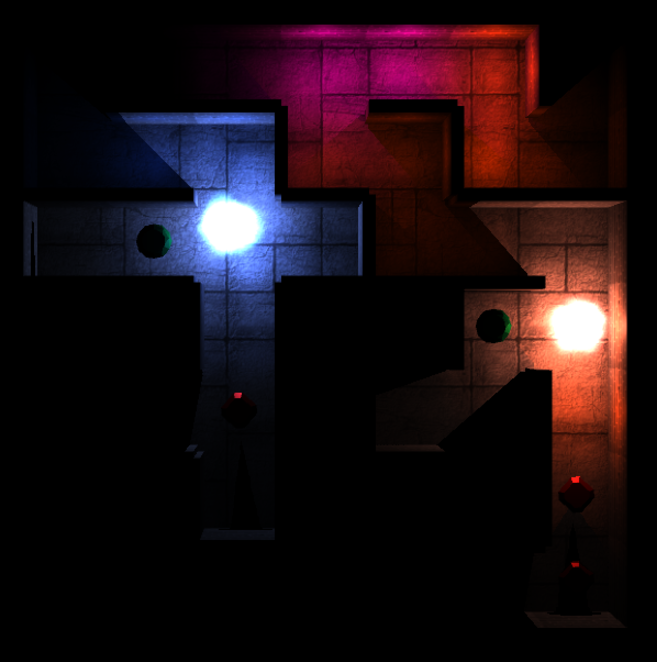
\includegraphics[width=0.9\columnwidth]{figures/maze}
  \caption{Two players surrounded by good and bad power-ups. The blue and orange parts are the players' private areas while the top right area is shared between both. }~\label{fig:figure1}
\end{figure}
\section{Implementation}
\subsection{Hardware}
We used the pupil framework developed by pupil labs \cite{kassner2014pupil} for this project. Pupil is an open source platform for mobile eye tracking and can be used for a variety of mobile eye tracking applications. Although the software has its bugs as we had to experience firsthand, it is still a lot more sophisticated than it was some years ago and tracking performance is really good. The headset consists of two cameras. One front facing webcam is capturing what is in the view of the user. A second smaller camera is located slightly below one eye and captures the whole eye. The software extracts the pupil from this image of the eye. The framework comes with a set of calibration methods that provide a way to map eye positions to points in the world view camera image. A user of the platform can easily add new plug-ins such as surface tracking or network capabilities to the basic pupil capture application. Some issues we discovered with the software and hardware were that the eye camera quickly gets very hot and needs to cool down. Also, the cameras are quite frequently not recognized by windows and drivers need to be reinstalled. The calibration sometimes crashes the application while other times the user's pupil can't be recognized reliably.

\subsection{Software}
The main crux in this project was developing a software system that integrates well with the given hardware and is fun to play. Also, there should be some experimental aspects to the implementation. In the following, we will show how we achieved this by explaining the key components of the software. The whole application was built using the Unity game engine with the programming language C\#. Implementation and testing took place on regular windows machines. We used git as VCS and GitLab to host our code and track issues.

\subsubsection{Menu}
At the beginning of the game the user can choose between many game configurations. There are the options to start the game, quit the application, get some helpful information or open a settings panel. In this settings panel, the user can connect new clients to the application, disconnect connected clients and calibrate clients. When deciding to play a new game from the main menu, the user can choose a game configuration. They can choose the number of players, the number of rounds and the difficulty of the game (simple, medium or hard) which affects the size of the labyrinth. The game can be paused using a break button next to the maze. In this pause mode the game can be continued and also aborted by going back to the main menu. All these options can be selected with the mouse.

\subsubsection{Maze Generator} 
The maze is generated with a depth-first-search algorithm. First we generate an $n*m$ large matrix and in every step we build a wall from $x_{0}$ to $x_{n}$ and from $y_{0}$ to $y_{m}$. In the next step we generate a datatype Cell with four walls (north, south, east, west). Now we will chose a random start cell, and destroy a random wall which has not yet been destroyed from this cell and progress with depth-first-search in every cell of the matrix. You can solve this problem with a running time of $\mathcal{O}(n^2)$.

\subsubsection{Power-Ups} 
We distinguish between positive or good power-ups and negative or bad power-ups. The good power-ups are \textit{enlightenment, endurance} and \textit{show target}. \textit{Enlightenment} is a light explosion. If a player collects this power-up, a range of size $(maze\_width / 7) * (maze\_height / 7)$ around the player will light up for a few seconds. \textit{Endurance} is a power-up that causes the light path to be illuminated for an extended period of time. The power-up \textit{show target} triggers a light flash on the target for a split second, making it hard for opponent players who are not expecting this to notice it. The bad power-ups are \textit{dim, slowing} and \textit{darkness}. \textit{Dim} is the opposite of \textit{endurance}, so the the light path is lit for a shorter time, but only of the opponents. The power-up \textit{slowing} slows down opponent players irreversibly. \textit{Darkness} extinguishes all existing lights of the opponents. So, although we call those power-ups bad or negative, they all have an immediate positive effect for the player collecting them which was a delibarate design decision based on the recommendation of Dorr et al. to make actions automatic whenever possible. \cite{dorr2009gaze}

\subsubsection{Smart Player Controls} 
We quickly discovered that simply moving the player to the position of the mouse or gaze does not work very well because the player has to keep the cursor very close to his light souce all the time. Also, this would not look very good because the lights will constantly move along the walls. We therefore decided to implement smart player controls, which means that the light will move towards the position of the cursor, but not in a straight line but through the corridors of the maze. For example, if the cursor is around a corner, the light will first move horizontally and then vertically around the corner, but never diagonally directly towards the cursor. \\
We noticed another problem with gaze: Oftentimes, the gaze is not very accurate and jumps around quite a lot. When we receive the gaze data from the eye tracker we convert this information into a cell in the maze. However, instead of naively trying to move the light to this cell, we also look at the neighboring cells. For each of them, we compute a simple heuristic which says how likely it is that this is the intended cell that the user wants to move to  (see Figure~\ref{fig:figure2}). So, even if the gaze position jumps around the intended cell, our algorithm will always suggest the cell that makes the most sense to move towards. This was not trivial to implement and we did not know if it would actually work. However, when we tested this approach, we found that moving the light through the maze is a lot more efficient. Without this approach, oftentimes the light went back and forth or stood still for prolonged periods of time. Now, we can move the light through the maze almost without errors or pauses.\\
Currently, this simple heuristic only takes into consideration whether the actual gaze position is within reach for the player and the distance of the path to reach it. Even though this is so simple, the results have been quite impressive. Improving this heuristic further will probably lead to even better results.
\begin{figure}
\centering
  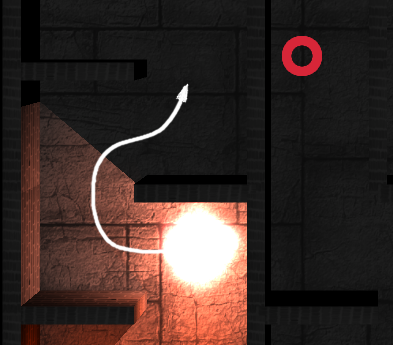
\includegraphics[width=0.9\columnwidth]{figures/algo}
  \caption{In this scenario, the player cannot reach the actual gaze position (red dot) and instead moves along the white arrow which is the path intended by the user. }~\label{fig:figure2}
\end{figure}
\subsubsection{Game Fairness}
We already mentioned the length of the path between two positions in the maze in the paragraph above. Obviously, getting this path is not straight-forward and the first time we felt that we need this functionality was when we wanted to spawn our target fair, such that all players have the same chance of reaching it first. In the first prototype, we used the simple Manhattan distance to find the position with roughly the same distance to all players. But of course, depending on the structure of the maze, this can lead to quite unfair target positions. We therefore implemented the A* search algorithm that takes two cells as input and returns the path (i.e. list of cells to visit) to get from the start cell to the end cell. By utilizing this, we can compute the spot in the maze which each player can reach in roughly the same time when making perfect decisions in choosing the way. We also introduce a lower bound on the length of the path to ensure that the target will not always spawn right between two players. When a new round starts, we generate new mazes until we find one where we can spawn the perfect target. When playing multiple rounds, we gradually make the spawning algorithm more liberal such that it will eventually spawn the target somewhere because we cannot generate a new maze in between rounds.

\subsubsection{Pupil Integration}
We created a class that stores the client information like IP addresses, ports and surface names. After those configurations have been read from the saved settings, we hand them over to the pupil listener. After validating the provided IP address and port, we establish a request socket and send a request for the sub port to the instance of pupil capture. 
\begin{verbatim}
requestSocket = new RequestSocket(
  IPHeader + c.port); 
requestSocket.SendFrame("SUB_PORT");)
\end{verbatim}

 After receiving this subport, we go on to set up the subscriber socket and subscribe to the surface and notify events of pupil capture. 
  \begin{verbatim}
 SubscriberSocket subscriberSocket = 
   new SubscriberSocket(header +  subport); 
subscriberSocket.Subscribe("surface");
subscriberSocket.Subscribe("notify.")
\end{verbatim}
 
We then enter a loop that continuously tries to read data from that socket.
 \begin{verbatim}
 bool stillAlive = subscriberSockets[turn].
  TryReceiveMultipartMessage(
    timeout, ref (msg));
\end{verbatim}

  Pupil provides this data as soon as it detects a defined surface within the view of the user. The message is a json file containing all sorts of information about the gaze and the surface. We extract the relevant information, which is whether the gaze is on the surface and the relative positions on the surface ranging from 0 to 1. This data is passed on to the gaze controller which converts this data into actual screen corrdinates which are then used to determine where to move the light. All of this is done in turn for all of the four players, meaning that data is fetched player-wise, one after another in quick succession. Thi is due to a restriction in unity that prevents us from receiving data from all four pupil instances concurrently. Still, this whole procedure is executed as a new thread so it does not block Unitys main UI thread.\\
Calibration is done in a similar fashion. When the calibration needs to be started, we send a request to the pupil client.
 \begin{verbatim}
sendRequest(requestSocket,
   new Dictionary<string, object> { 
     { "subject", "calibration.should_start" }, 
     { "marker_size", "1.50" }, 
     { "sample_duration", "50" } 
   }
);
\end{verbatim}

This starts the internal pupil screen marker calibration. We can then find out when the calibration is over by checking for each received message whether the message type equals a certain event id.
 \begin{verbatim}
if (msgType.Equals(
  "notify.calibration.successful")) {
    // end calibration }
\end{verbatim}

\subsubsection{Calibration}
In order to use the pupil trackers and have a good level of accuracy, a calibration that maps eye positions to locations in the view of the world camera is necessary. When a calibration is done, the tracker must not move on the players head. Otherwise, the slight shift will introduce a more or less severe offset which quickly leads to very bad usability. To account for that, we introduced a calibration procedure in our application. We decided to do this in a rather simple way: From the settings screen where we can connect to pupil clients, we can also choose to start the calibration procedure for each client. This will send a request to the client computer and start the pupil internal screen marker calibration procedure. Our game then listens for an event from pupil, indicating a successful or failed procedure. Furthermore, when a new game starts each player that has not been calibrated previously will be calibrated in the same way. When the calibration for every player is done, the players can join the game.

\subsubsection{Game Lobbys}
We implemented a very intuitive and efficient way for gaze players to join a new game. Because our maximum number of players is four, we divided the screen into four areas. When a player gazes at one of those areas, a countdown from 3 to 0 is shown to indicate how long they have to keep looking there to join. After all players have joined in that manner, the game will start automatically  (see Figure~\ref{fig:figure3}). To ensure that games don't get empty, we implemented the possibility for mid-game joining. When players are inactive, i.e. they do not gaze at the screen for a certain number of seconds, they will be kicked out of the game. New players can then join the ongoing game in the same manner as described above, with the only difference that the other players can keep on playing. The new player will then join the game and spawn when the next round starts. 
\begin{figure}
\centering
  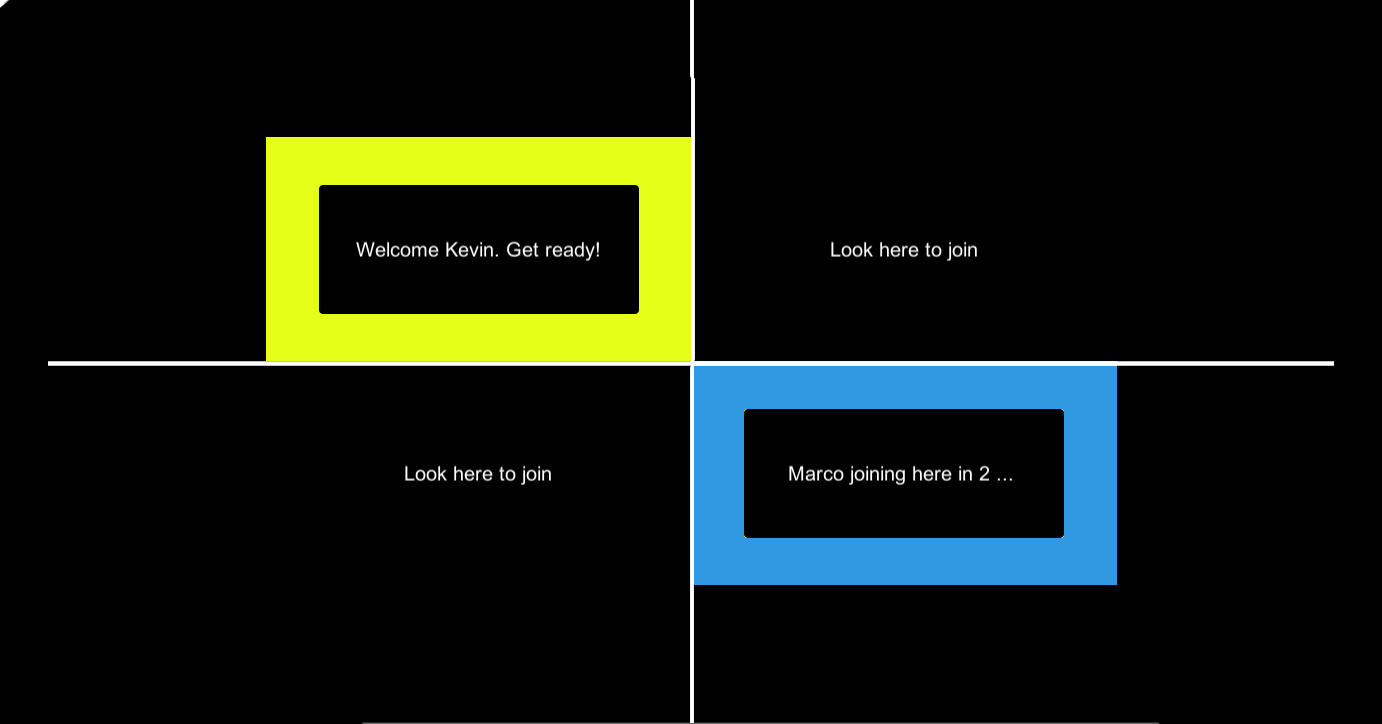
\includegraphics[width=0.9\columnwidth]{figures/join}
  \caption{The join screen. The yellow player has joined at the top left while the blue player will join at the bottom right in two seconds. The other two spots are free for two more gaze players. }~\label{fig:figure3}
\end{figure}
\subsubsection{Graphical Interface} 
To get an immersive game experience we integrated special effects and high quality 3D objects. The special effects which we took from a collection of particle systems from the asset store occur in many places in the game. Among the many alternatives, we chose two effects for our power-ups that fit quite well, one for the good and one for the bad power-ups. We changed some parameters of these effects (i.e the loop, the color, initial size and behaviour over time). They are triggered as soon as a user collects a power-up. To make the game more interesting, we integrate fog. The fog spawns randomly and grows as the game progresses. The fog has the color of the player in lead. This way, players do not have to look at the scoreboard but can continue to focus on the game. The fog introduces visual complexity, which Dorr et al. found out can make a game more challenging and fun to play for gaze players. \cite{dorr2009gaze} .\\
Power-ups and the target are displayed as gems which we also took from the asset store. We choose 3 different gems to distinguish the target and the two power-up types  (see Figure~\ref{fig:figure4}). The player character itself is a rather nice looking particle effect.
\begin{figure}
\centering
  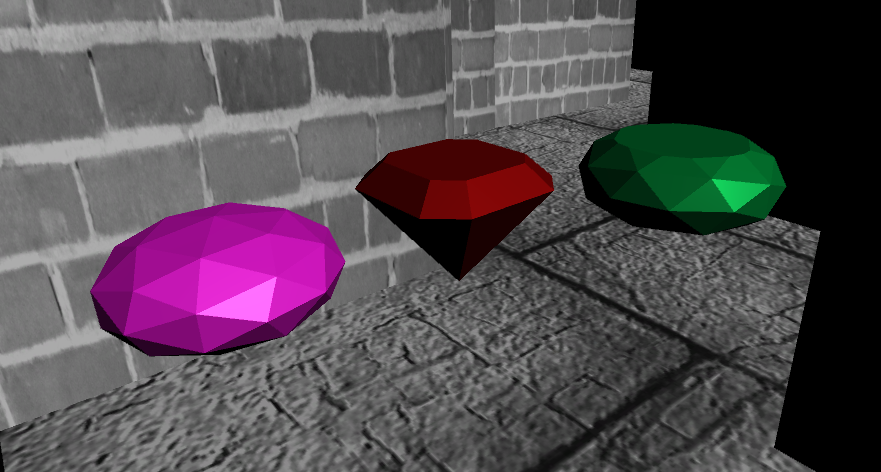
\includegraphics[width=0.9\columnwidth]{figures/gems}
  \caption{Power-ups and the target are valuable gems. From left to right: target, negative power-up, positive power-up}~\label{fig:figure4}
\end{figure}

\section{Evaluation}
\subsection{Performance}
We tested and played the game a lot of times and it turned out that the performance of gaze players is very good. We can move through the maze with close to zero errors. However, this is highly correlated to the accuracy of the tracker. When the calibration is not done properly or the tracker moved on the user's head, introducing a significant offset, the game can quickly become extremly hard and frustrating to play. When we first integrated the tracker into our game, it was quite hard to navigate through the maze. However, as we tried out different ideas, we managed to improve performance and efficiency quite a lot. Of course, this is just a subjective opinion and us becoming more used to the eye tracker over time certainly also played a role. The next step would be to conduct a controlled experiment where we compare performance using different gaze estimation and optimization techniques as well as a direct comparison between mouse and gaze. A tournament as Dorr et al. \cite{dorr2009gaze} did would be a fun way to do this.

\subsection{User-Experience}
We did a very small subjective evaluation where we interviewed some friends, none of which has used eye tracking before. Because of that, they needed some time to get used to the eye tracker and the game. Still, they quickly got used to the tracker and managed to confidently light up their way through the maze. We also got very positive feedback regarding the overall interface and graphics of the game. Most people liked the effects quite a lot and found the music that builds tension quite fitting. Also, the interplay of the different colors is quite interesting to observe as a non-player. Overall, we are more than pleased with the reactions and even received valuable suggestions for improvement.

\section{Conclusion}
\subsection{R{\'e}sume}
Subject of this project was to design and implement a multi-user gaze-based game with special focus of incorporating content adaption into the design of the game. By developing this game, we created a proof-of-concept that a game that is controled solely using gaze interaction does not have to be frustrating. By deliberately making decisions based on ideas from other researchers and trying out new approaches to make the interaction easier, we discovered that playing a game using gaze can actually be a lot of fun. Even more, we found ways how we can adapt content such that multiple users can play together on one screen.

\subsection{Lessons Learned}
The main benefit of having done this project is that we have learned a lot of important lessons. Besides lessons in project management and software engineering practices, we will explain the key insights related to gaze interaction. While some of them were already mentioned in related work, we also gained some new ideas from our unique approach and experimentation with different settings and implementations. We would like to present those findings as guidelines for others to implement in their eye tracking projects.
 \begin{itemize}
\item Make hit areas bigger than visual parts.
\item Use more than four markers and make them as small as possible and as big as necessary to increase stability and precision
\item Accurate tracking is important and offsets are frustrating. Do not show the actual gaze position as cursor whenever possible.
\item Make actions automatic whenever possible.
\item Use two modes for player control and scanning. This can be achieved by defining a fixed radius around the player where movement is possible.
\item Estimate the best user gaze position. Do not take the raw gaze data but find a heuristic that yields a better estimate of what the user intends to do in the given state of the game.
\item Introduce visual complexity to challenge gaze players. Visual polish is very important  (see Figure~\ref{fig:figure5}).
\end{itemize}
\begin{figure}
\centering
  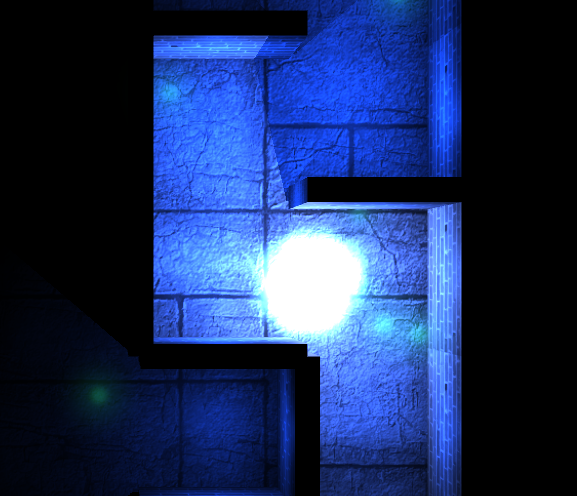
\includegraphics[width=0.9\columnwidth]{figures/visuals}
  \caption{A player collecting a positive power up. Effects and high quality graphics will catch the user's eye.}~\label{fig:figure5}
\end{figure}

\subsection{Future Work}
In general, there are many possibilities to extend Maze Gaze. Instead of controlling the menu by mouse we could implement a menu that can be controlled by gaze. However, this should not be done by selecting buttons but rather a by moving of the light to certain areas to select the game configuration. This would introduce the user to the game and be a lot more intuitive than selecting buttons.\\ 
We also could create a collaborative team mode so that two players are in one team and other two players are in a opponent team. The teams have to play against each other. That means, if a player of the one team collects a bad power-up it just will be triggered on the members of the other team and not for the player of the own team.\\ 
Another idea would be to change the maze during play time, just ike the game ''Labyrinth'' from Ravensburger from the year 1986. An algorithm could destroy walls and build up other walls while keeping the maze fair and all spots reachable. This ensures that the users can not only rely on their memory, but also a luck factor plays a role.\\
Besides those gameplay improvements, there are also many things we can add related to the eye trackers. One point is the continuation and improvement of the calibration. We could move the calibration from the client machine into our game, such that the calibration will start on the desktop where the game is running and not where pupil is running. We also could implement an in-application pursuit calibration to get a more precise calibration and better user experience. Another rather simple idea that we did not have the time to implement is to create our own simple calibration on top of the pupil calibration that would get rid of constant offsets by simply shifting every position into a certain direction to match it with the actual gaze position again. \\ 
To reduce the frustration of the user, we could improve the gaze precision. The gaze precision is currently good enough to have a good gaming experience without major frustrations but not perfect yet. The improvement is possible by applying algorithms to the actual gaze position to calculated to the desired position. Also, smoothing of gaze values can be incorporated. \\
\\
To wrap things up, having faced and courageously overcome several challenges, we are pleased to deliver an application that fulfills the initial requirements and expectations. The lessons we learned can help other developers to create similar multi-user gaze-based games where content adaption is useful. It is in our interest to develop this prototype further and test different hypotheses in experiments and user studies. Having done this initial research and work, we have also set the cornerstone for further development and research, which will hopefully inspire others and eventually contribute to the design of great games using gaze-interaction.

\balance{}


% REFERENCES FORMAT
% References must be the same font size as other body text.
\bibliographystyle{SIGCHI-Reference-Format}
\bibliography{sample}

\end{document}

%%% Local Variables:
%%% mode: latex
%%% TeX-master: t
%%% End:
